\documentclass[a4paper,11pt,wide]{scrartcl}
\usepackage[top=2.5cm, bottom=2.5cm, left=2.5cm, right=2.5cm]{geometry}

\usepackage{pgf}
\usepackage{tikz}
\usetikzlibrary{arrows,automata}

\usepackage[latin1]{inputenc}

\title{Test}

\begin{document}


\maketitle

\section{Content}
Test

\section{Parameters}

\subsection{Wait Data Timeout}
Timeout after Trigger is received before first data arrives

\subsection{Send Data Timeout}
Timeout after package is started, while there is no data in the
package fifos

\subsection{Packet size}

Max number of words in a GBT packet. If this is saturated, the packet
is closed and a new packet opened.

\section{Data fields}
\subsection{SOP}
\subsection{EOP}
\subsection{CDH}
\begin{verbatim}
CDH0
  zero(24bit) & priority(8bit) & FEE ID(16bit) &
  block length(16bit) & header size(8bit) & header version(8bit)
CDH1
  zero(16bit) & HB Orbit (32bit) & TRG Orbit(32bit)
CDH2
  zero(16bit)  & TRG Type (32bit) & zero(4bit) & HB BC (12bit) &
  zero(4bit) & TRG BC (12bit)
CDH3
  zero(24bit) & Pages Counter (16bit) & STOP (8bit) & PAR (16bit) & Det Field (16bit)
\end{verbatim}
\subsection{Header}
\begin{tabular}[htb]{r|r|l|l}
  Position & Width & Name & Desctiption \\
  \hline
  79 : 72 & 8 & xE0 (header indicator) \\
  71 : 44 & - & Not defined & - \\
  43 : 16 & 28 & active\_lanes & Number of lanes active (eligible for
                                  readout) \\
  15 : 0 & 16 & packet\_idx & Index of GBT packet within trigger \\
\end{tabular}
\subsection{Data}
\begin{tabular}[htb]{r|r|l|l}
  Position & Width & Name & Desctiption \\
  \hline
  79 : 72 & 8 & lane\_idx & Lane Index \\
  71 : 0  & 72 & lane\_data & Lane Data
\end{tabular}
\subsection{Trailler}
\begin{tabular}[htb]{r|r|l|l}
  Position & Width & Name & Desctiption \\
  \hline
  79 : 72 & 8 & xF0 (trailer indicator) \\
  71 : 64 & 8 & packet\_state & State of packager \\
   & 4 & lane\_timeouts & 1 if at least 1 lane timed out \\
   & 3 & lane\_starts\_violation & 1 if at least 1 lane had a start violation \\
   & 2 & max\_packets\_reached & Packet overflow: Max number of packets reached \\
   & 1 & transmission\_timeout & Timeout of transmission (lanes)\\
   & 0 & packet\_done & Packet finished \\
  63 : 60 & 4 & - & not used \\
  59 : 32 & 28 & vlane\_timeout & Lane timeouts received \\
  31 : 28 & 4 & - & not used \\
  27 : 0 & 28 & vlane\_stops & Lane stops received \\
\end{tabular}
\section{Statemachine}

\resizebox{!}{.9\textheight}{
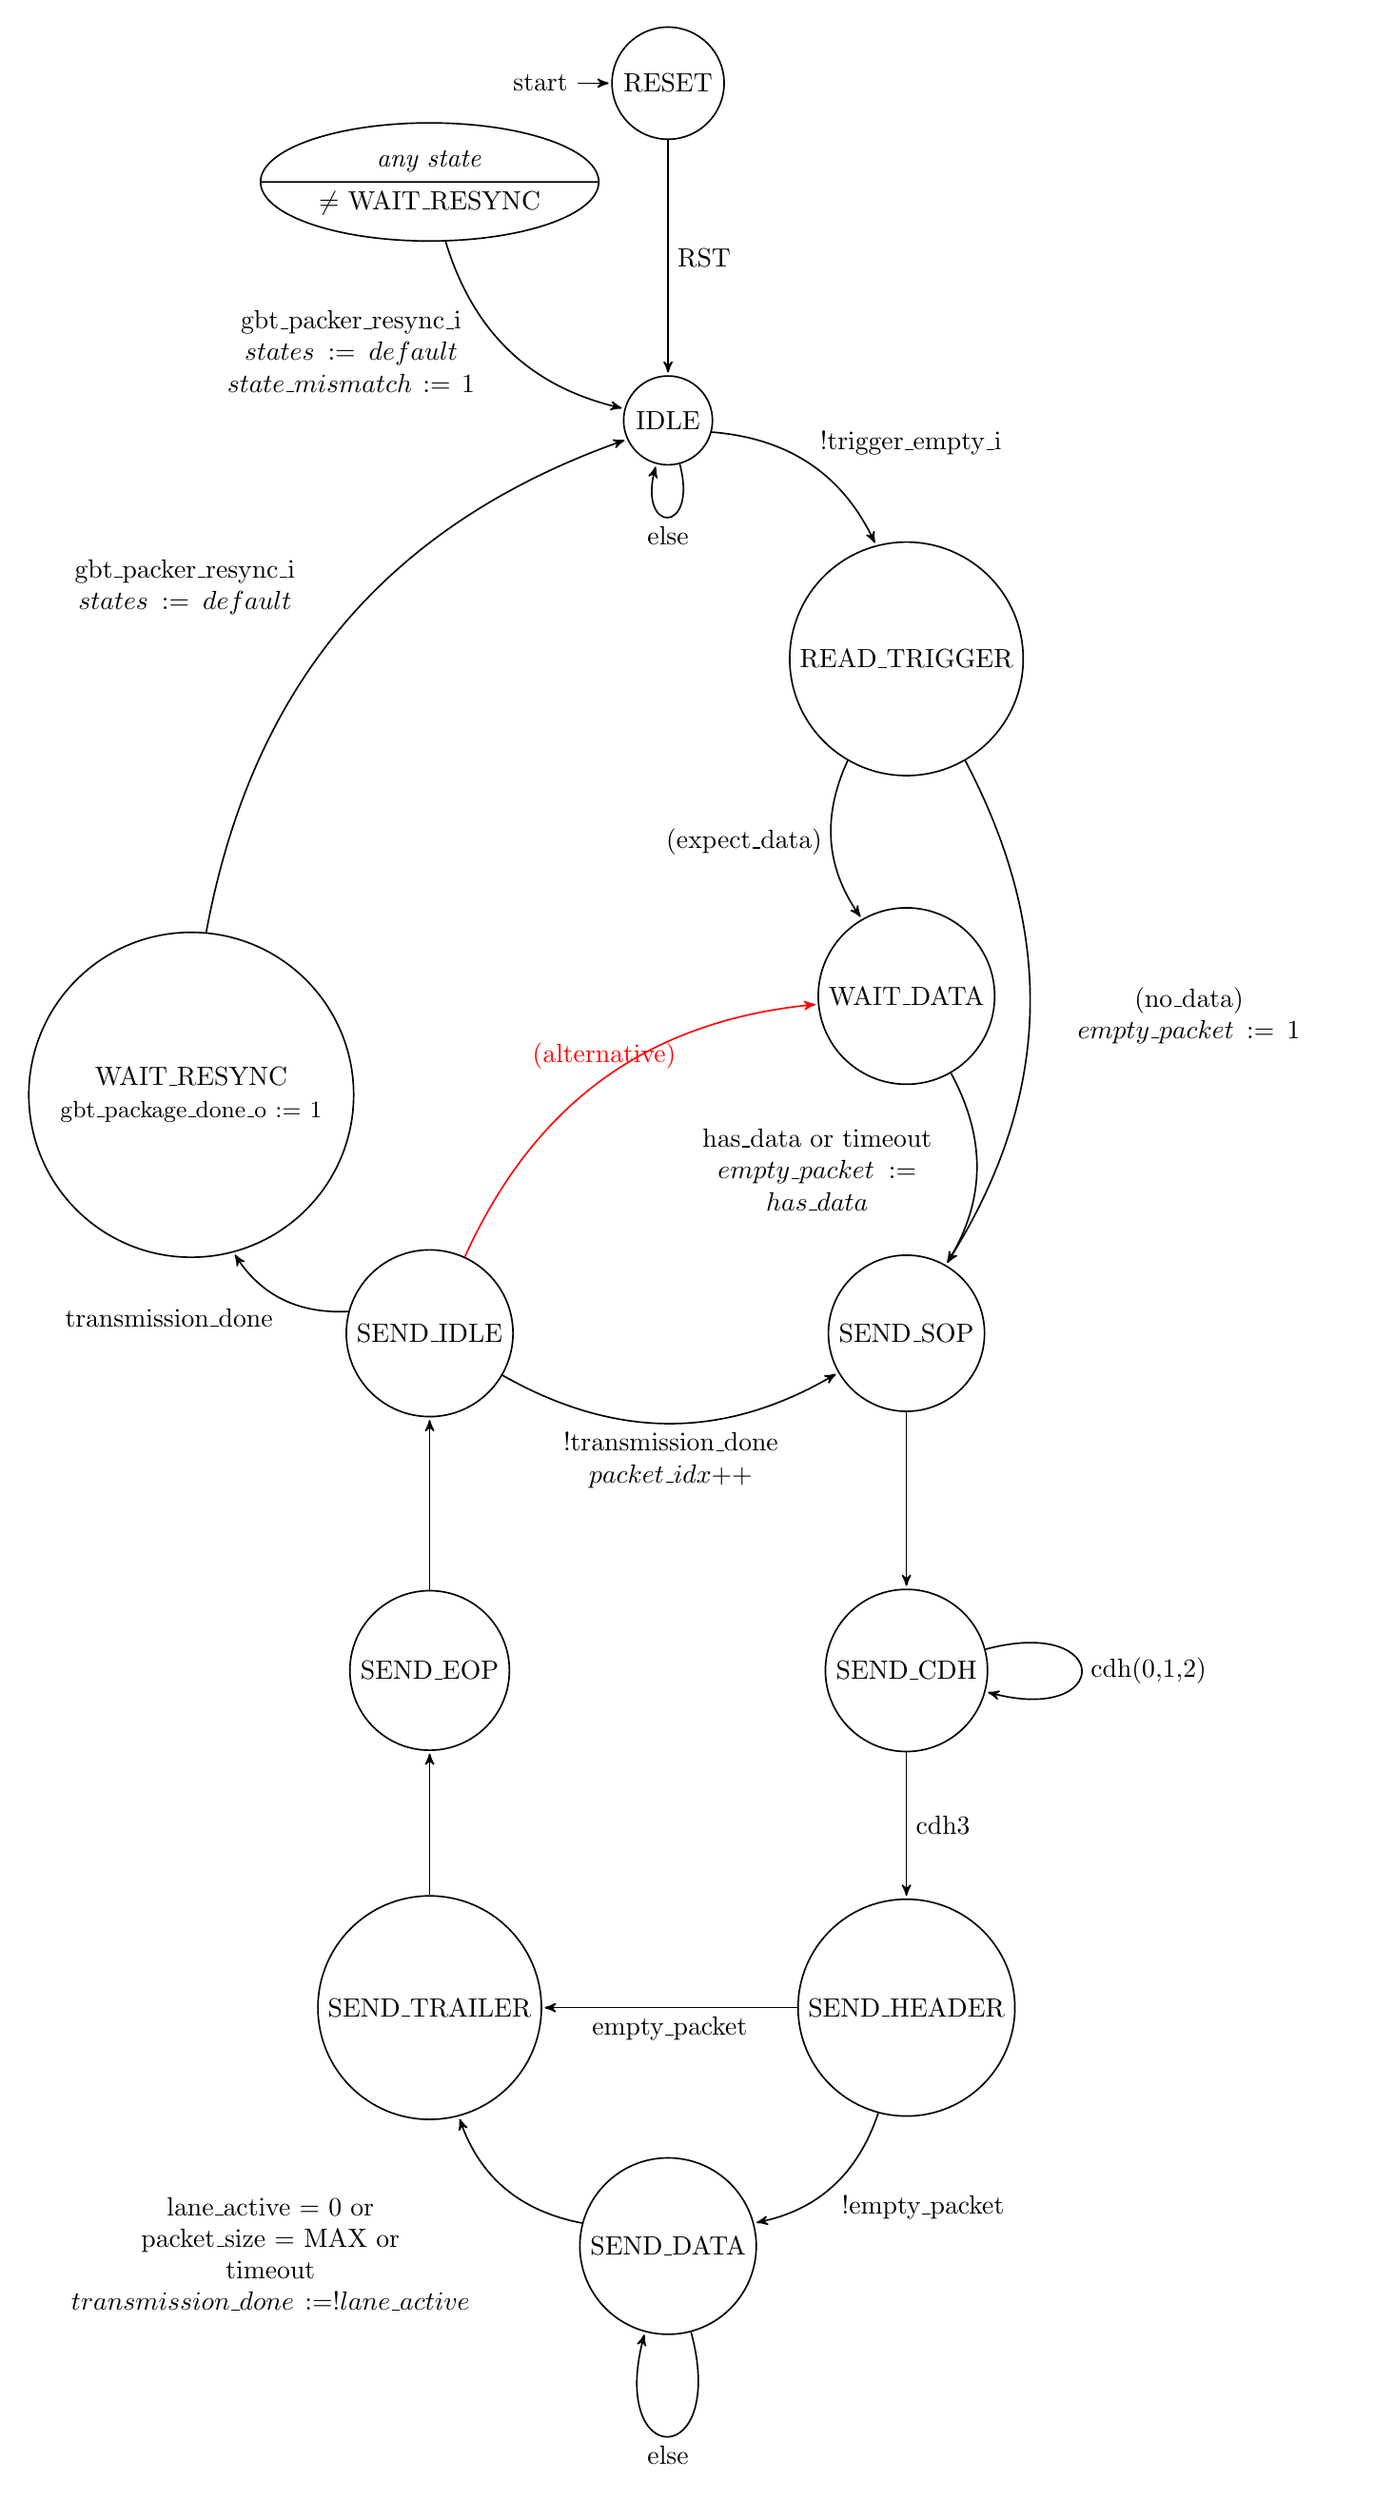
\begin{tikzpicture}[->,>=stealth',shorten >=1pt,auto,node distance=4.5cm,
                    semithick]
  \tikzstyle{every state}=[draw=black,text=black]
  \node[initial,state] (RST) {RESET};
  \node[state]         (ID) [below of=RST]{IDLE};
  \node[state]         (RT) [below right of=ID] {READ\_TRIGGER};
  \node[state]         (WD) [below of=RT] {WAIT\_DATA};
  \node[state]         (SS) [below of=WD] {SEND\_SOP};
  \node[state]         (SC) [below of=SS] {SEND\_CDH};
  \node[state]         (SH) [below of=SC] {SEND\_HEADER};
  \node[state]         (SD) [below left of=SH] {SEND\_DATA};
  \node[state]         (ST) [above left of=SD] {SEND\_TRAILER};
  \node[state]         (SE) [above of=ST] {SEND\_EOP};
  \node[state]         (SI) [above of=SE] {SEND\_IDLE};
  \node[state]         (WR) [above left of=SI, text width=4cm, align=center]
  {WAIT\_RESYNC\\ \small{gbt\_package\_done\_o := 1}};
  \node[state, ellipse split]         (ANY) [above left
  of=ID] {\emph{any state} \nodepart{lower} $\neq$ WAIT\_RESYNC};

\path (RST) edge node {RST} (ID)
      (ID)  edge [bend left] node {!trigger\_empty\_i} (RT)
            edge [loop below] node {else} (ID)
      (RT) edge [bend right,left] node {(expect\_data)} (WD)
      (RT) edge [bend left,text width=4cm,align=center] node {(no\_data)\\$empty\_packet:=1$} (SS)
      (WD) edge [bend left,text width=4cm,align=center,left] node
      {has\_data or timeout\\$empty\_packet:=has\_data$} (SS)
      (SS) edge [] node {} (SC)
      (SC) edge [] node {cdh3} (SH)
           edge [loop right] node {cdh(0,1,2)} (SC)
      (SH) edge [bend left] node {!empty\_packet} (SD)
      (SH) edge [] node {empty\_packet} (ST)
      (SD) edge [loop below] node {else} (SD)
      (SD) edge [bend left,text width=6cm,align=center] node {lane\_active = 0 or\\
        packet\_size = MAX or\\ timeout\\$transmission\_done := !lane\_active$} (ST)
      (ST) edge [] node {} (SE)
      (SE) edge [] node {} (SI)
      (SI) edge [bend left] node {transmission\_done} (WR)
      (SI) edge [bend right,below,text width=4cm,align=center] node
      {!transmission\_done\\$\mathrel{packet\_idx}\mathrel{+}\mathrel{+}$}
      (SS)
           edge [above,bend left,color=red] node {(alternative)} (WD)
      (WR) edge [bend left,text width=4cm,align=center] node
      {gbt\_packer\_resync\_i\\$states:=default$} (ID)
      (ANY) edge [bend right,left,text width=4cm,align=center]
      node {gbt\_packer\_resync\_i\\$states:=default$\\$state\_mismatch:=1$} (ID);

\end{tikzpicture}
}% resizebox

\end{document}

%%% Local Variables:
%%% mode: latex
%%% TeX-master: t
%%% End:
